\item \points{2f} {\bf Overfitting with expressive models and small data}

You will not be required to code, write, or submit anything for this sub-question.  For this and the remaining sub-questions, we will consider a small
dataset (a random subset of the dataset you have been using so far) with much fewer examples, provided in
the following file:
%
\begin{center}
	\texttt{src/small.csv}
\end{center}
%

We will be exploring what happens when the number of features start becoming bigger than the number of 
examples in the training set. Run your algorithm on this small dataset using the following feature map 
\begin{align}
\phi(x) = \left[\begin{array}{c} 1\\ x \\ x^2\\ \vdots \\x^k \end{array}\right]\in \mathbb{R}^{k+1} 
\end{align}
with $k = 1,2,3,5,10,20$ using the autograder test case |2f-0-basic|, which will create plots in |src/smalle-poly.png| and |src/small-sine.png|. 

\textbf{Remark: } The phenomenon you observe where the models start to fit the training dataset very well, but suddenly ``goes wild'' is due to what is called \emph{overfitting}. The intuition to have for now is that, when the amount of data you have is small relative to the expressive capacity of the family of possible models (that is, the hypothesis class, which, in this case, is the family of all degree $k$ polynomials), it results in overfitting.  

Loosely speaking, the set of hypothesis function is ``very flexible'' and can be easily forced to pass through all your data points especially in unnatural ways. In other words, the  model explains the noises in the training dataset, which shouldn't be explained in the first place. This hurts the predictive power of the model on test examples. We will describe overfitting in more detail in future lectures when we cover learning theory and bias-variance tradeoffs.\\

Your plots should look similar to the following:
\begin{figure}[H]
  \centering
  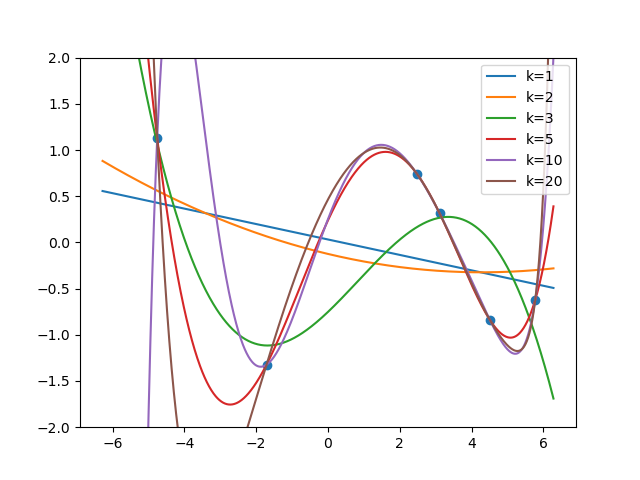
\includegraphics[width=0.65\linewidth]{02-featuremaps/small-poly.png}
  \caption{Polynomial regression with kernel sizes 1,2,3,5,10 and 20
  on small dataset}
  
  \centering
  \vspace{2mm}
  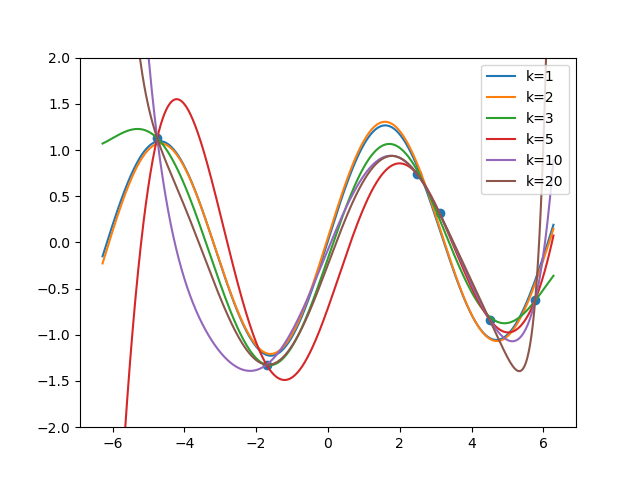
\includegraphics[width=0.65\linewidth]{02-featuremaps/small-sine.png}
  \centering
  \caption{Regression with other polynomial and sinusoidal features with kernel sizes 1,2,3,5,10 and 20
  on small dataset}
\end{figure}
